% \documentclass[a4paper, 10px]{ctexart}
\documentclass{ctexart}
\usepackage[left=1in, right=1in, top=1.2in, bottom=1.2in]{geometry}
\usepackage{ctex}
\usepackage[utf8]{inputenc}
\usepackage{boxproof}
\usepackage{tikz}
\usetikzlibrary{automata}
\usepackage{fontspec}
\usepackage{a4wide}
% \setmainfont[Scale = 1]{Palatino}
% \setCJKmainfont{Songti SC}
\usepackage{fancyhdr}
\pagestyle{fancy}
\fancypagestyle{plain}{
    \fancyhead[L]{East China Normal University}
    \fancyhead[R]{}
    \fancyfoot[C]{\thepage}
}
\def\premise{\mathrm{premise}}
\def\assumption{\mathrm{assumption}}
\def\MT{\mathrm{MT\ }}
\def\LEM{\mathrm{LEM}}
\def\intro{\mathrm{i\ }}
\def\elim{\mathrm{e\ }}
\def\introa{\mathrm{i_1\ }}
\def\elima{\mathrm{e_1\ }}
\def\introb{\mathrm{i_2\ }}
\def\elimb{\mathrm{e_2\ }}

\title{Logic in Computer Science Assignment 1}
\author{10185101210 陈俊潼}
\date{September 2020}

\begin{document}

\maketitle

\section{证明}

\subsection{$\neg (p \wedge q) \dashv \vdash \neg q \vee p)$}
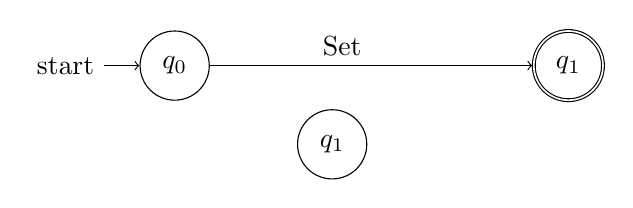
\begin{tikzpicture}[]
    \node[state, initial](q0) {$q_0$};
    \node[state](q1) at (2,-1) {$q_1$};
    \node[state, accepting](q2) at (5,0) {$q_1$};
    \path[->] (q0) edge node [above left] {Set} (q2);
    \end{tikzpicture}

\newpage
\subsection{\(p \rightarrow q \dashv\vdash \neg q \rightarrow \neg p\)}

正向:
$$
% \proofboxformulawidth=18em\relax
\begin{proofbox}
   \: p\to q \= \premise\\
      \[
         \: \neg q \= \assumption\\
         \: \neg p \=  \MT1,2\\
      \]
   \: \neg q\to\neg p \= \to\intro2-3\\
\end{proofbox}$$
逆向:
$$
\begin{proofbox}
   \: \neg q\to\neg p \= \premise\\
      \[
         \: p \= \assumption\\
         \: \neg\neg p \= \neg\neg\intro2\\
         \: \neg\neg q \=  \MT1,3\\
         \: q \= \neg\neg\elim4\\
      \]
   \: p\to q \= \to\intro2-5\\
\end{proofbox}$$

\subsection{\(p \wedge q \rightarrow p \dashv\vdash r \vee \neg r\)}

正向:
$$
% \proofboxformulawidth=18em\relax
\begin{proofbox}
   \: r\vee\neg r \= \LEM
\end{proofbox}$$
逆向:
$$
\begin{proofbox}
   \[
      \: p\land q \= \assumption\\
      \: p \= \land\elima1\\
   \] 
\: p\land q\to p \= \to\intro1-2\\
\end{proofbox}$$
\end{document}
